\usetikzlibrary{arrows.meta,calc}
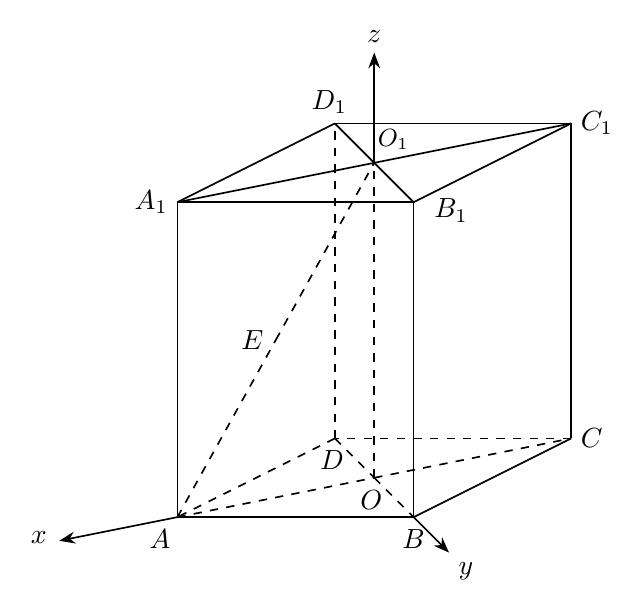
\begin{tikzpicture}[x=1cm,y=1cm,line width=.6pt,font=\normalsize]
\tikzset{ptlabel/.style={font=\normalsize,fill=white,inner sep=1.2pt}}
% Oblique projection of straight rhombic prism, schematic layout matching original PNG
\coordinate (A) at (0,0);
\coordinate (B) at (3,0);
\coordinate (C) at (5,1);
\coordinate (D) at (2,1);
\coordinate (A1) at (0,4);
\coordinate (B1) at (3,4);
\coordinate (C1) at (5,5);
\coordinate (D1) at (2,5);
\coordinate (O) at (2.5,0.5);
\coordinate (O1) at (2.5,4.5);
\coordinate (E) at (1.25,2.25);
\coordinate (Xend) at (-1.5,-0.3);
\coordinate (Yend) at (3.45,-0.45);
\coordinate (Zend) at (2.5,5.9);
% bottom face: front solid, back dashed
\draw (A) -- (B);
\draw (B) -- (C);
\draw[dashed] (C) -- (D);
\draw[dashed] (D) -- (A);
% bottom diagonals dashed
\draw[dashed] (A) -- (O);
\draw[dashed] (O) -- (C);
\draw[dashed] (D) -- (O);
\draw[dashed] (O) -- (B);
% verticals
\draw (A) -- (A1);
\draw (B) -- (B1);
\draw (C) -- (C1);
\draw[dashed] (D) -- (D1);
\draw[dashed] (O) -- (O1);
% top face solid
\draw (A1) -- (B1);
\draw (B1) -- (C1);
\draw (C1) -- (D1);
\draw (D1) -- (A1);
% top diagonals solid crossing at O1
\draw (A1) -- (C1);
\draw (D1) -- (B1);
% space diagonal A-O1 dashed with midpoint E
\draw[dashed] (A) -- (E);
\draw[dashed] (E) -- (O1);
% axes arrows from A (x), B (y), O1 (z)
\draw[-{Stealth[length=2mm]}] (A) -- (Xend);
\draw[-{Stealth[length=2mm]}] (B) -- (Yend);
\draw[-{Stealth[length=2mm]}] (O1) -- (Zend);
% labels with white background and offset to avoid touching strokes
\node[ptlabel,below left,xshift=-1pt,yshift=-1pt,fill=none,xshift=0.00bp,yshift=-2.00bp] at (A) {$A$};
\node[ptlabel,below,xshift=2pt,yshift=-3pt,fill=none,xshift=-2.00bp,yshift=0.00bp] at (B) {$B$};
\node[ptlabel,right,xshift=2pt] at (C) {$C$};
\node[ptlabel,below,xshift=-1pt,yshift=-3pt,fill=none] at (D) {$D$};
\node[ptlabel,left,xshift=-2pt] at (A1) {$A_{1}$};
\node[ptlabel,right,xshift=2pt,yshift=1pt,fill=none,xshift=4.00bp,yshift=-4.00bp] at (B1) {$B_{1}$};
\node[ptlabel,right,xshift=2pt] at (C1) {$C_{1}$};
\node[ptlabel,above,xshift=-2pt,yshift=2pt] at (D1) {$D_{1}$};
\node[ptlabel,below,xshift=1pt,yshift=-3pt,fill=none,xshift=-2.00bp,yshift=0.00bp] at (O) {$O$};
\node[ptlabel,font=\small,anchor=west,fill=none,inner sep=1pt,xshift=0.0bp,yshift=1.0bp] at (2.5,4.76) {$O_{1}$};
\node[ptlabel,left,xshift=-3pt] at (E) {$E$};
\node[ptlabel,left,xshift=-3pt,yshift=1pt] at (Xend) {$x$};
\node[ptlabel,below right,xshift=2pt,yshift=-2pt] at (Yend) {$y$};
\node[ptlabel,above,yshift=2pt] at (Zend) {$z$};
\end{tikzpicture}
